\documentclass[10pt,landscape,twocolumn]{article}

\usepackage{lscape}
\usepackage[english]{babel}
\usepackage[utf8]{inputenc}
\usepackage{fullwidth}

\usepackage{tikz}
\usetikzlibrary{shapes}
\usetikzlibrary{calc}
\usepackage{fancyhdr}
\pagestyle{fancy}

\usepackage{algorithmicx}
\usepackage{algpseudocode}

\renewcommand{\footrulewidth}{1pt}
\fancyfoot[C]{\thepage}

\renewcommand{\headrulewidth}{1pt}
\fancyhead[L]{ACM ICPC}

\begin{document}

\begin{center}
	\Large ICPC Training Material : Data Structures, Algorithms and Theorems 
\end{center}

\tableofcontents

\section{Data Structures}

\subsection{Elementary Data Structures}
In Computer Science, in order to treat and store data, it first needs to be structured. Hence, multiple data structures were created : Array, Hash, Queue, Tree and multiple others.

\subsubsection{Array}
The array is the most used data structure. It consists on a collection of values, such as each value is identified by at least one index. 

\begin{center}
	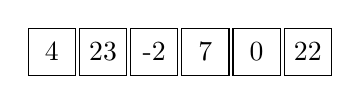
\begin{tikzpicture}
	\coordinate (s) at (0,0);
	\foreach \num in {4,23,-2,7,0,22}{
		\node[minimum size=6mm, draw, rectangle] at (s) {\num};
		\coordinate (s) at ($(s) + (0.65,0)$);
	}
	\end{tikzpicture}
\end{center}
Arrays are useful because they exploit the addressing logic of computers. Generally, the memory is a one-dimensionnal array of words, whose indices are the addresses. 


\subsubsection{Linked List}

The linked list is a linear data structure in which the objects are ordered according to the value of their pointer. \\

Every object $x$ of the linked list $L$ has a key attribute $x.key$ and a successor $x.succ$ attribute.

\begin{center}
	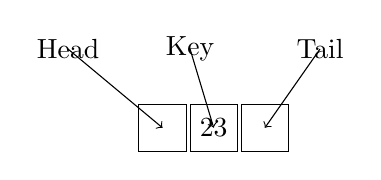
\begin{tikzpicture}
	\coordinate (s) at (0,0);
	\node[minimum size=6mm, draw, rectangle] at (s) {};
		\coordinate (h) at ($(s) +  (-1.2,1)$);
		\node[draw=none,fill=none] at (h) {Head};
		\draw[->] (h.south east) -- (s.north west);
		\coordinate (s) at ($(s) + (0.65,0)$);
	\node[minimum size=6mm, draw, rectangle] at (s) {23};
		\coordinate (k) at ($(s) + (-0.3,1)$);
		\node[draw=none,fill=none] at (k) {Key};
		\draw[->] (k.south) -- (s.north);
	        \coordinate (s) at ($(s) + (0.65,0)$);
	\node[minimum size=6mm, draw, rectangle] at (s) {};
		\coordinate (t) at ($(s) + (0.7,1)$);	
		\node[draw=none,fill=none] at (t) {Tail};
		\draw[->] (t.south west) -- (s.north east);	
		\coordinate (s) at ($(s) + (0.65,0)$);
	\end{tikzpicture}
\end{center}

In the case of double linked lists, a $x.prec$ attribute is added. An exemple is given below : \\


	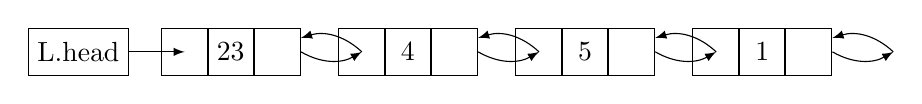
\begin{tikzpicture}[scale=0.9]
	\coordinate (s) at (1.5,0);
	\node[minimum size=6mm, draw] (h) at (0,0) {L.head};
	\draw[->,>=latex] (h)  to [right] (s);
	\foreach \num in {23,4,5,1}{
		\node[minimum size=6mm, draw, rectangle] (p1) at (s) {};
		\coordinate (s) at ($(s) + (0.65,0)$);
		\node[minimum size=6mm, draw, rectangle] (p1) at (s) {\num};
		\coordinate (s) at ($(s) + (0.65,0)$);
		\node[minimum size=6mm, draw, rectangle] (p1) at (s) {};
		\coordinate (s) at ($(s) + (1.2,0)$);
		\draw[->,>=latex] (p1.east) to [bend right] (s.west);
		\draw[->,>=latex] (s.west) to [bend right] (p1);
	}
	\end{tikzpicture} \\

In the case of a circular list, the attribute $x.prec$ at the queue of the list points at the head, and the attribute $x.succ$ at the head of the list points at the tail. Hence, the list can be seen as a \textbf{ring} of elements.\\

Linked List provide the advantage of having a dynamic size, as in an rray memory is allocated during compilation time while it is allocated at runtime for linked lists.\\ 

\subsubsection{Stack}

The stack consists on a collection of data that is added and retrieved according to the FILO(First In Last Out) method.

Two operations, which can only be applied on the top element of the stack, are used to manipulate the data :
\begin{itemize}
	\item Push : Used to add a block on the top of the stack. A stack is overflowed if the number of blocks exceeds the capacity.  
	\item Pop : Used to retrieve the block at the top of the stack.
\end{itemize}

\begin{center}
	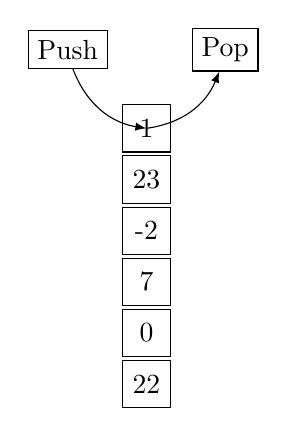
\begin{tikzpicture}
	\coordinate (s) at (0,0);
	\node[draw, rectangle] (po) at (1,1) {Pop};
	\node[draw, rectangle] (pu) at (-1,1) {Push};
	\draw[->,>=latex] (s.east) to[bend right] (po);
	\draw[->,>=latex] (pu) to[bend right] (s.west);
	\foreach \num in {1,23,-2,7,0,22}{
		\node[minimum size=6mm, draw, rectangle] at (s) {\num};
		\coordinate (s) at ($(s) - (0,0.65)$);
	}
	\end{tikzpicture}
\end{center}

An intuitive application would be inversing strings or numbers. It is also used for memory management, as well as in expression evaluation. Stacks are implemented using arrays or linked lists, the two previous data structures.

\subsubsection{Queue}


\subsubsection{Heap}
\subsubsection{Hash}
\subsubsection{Trees}

\subsection{Advanced Data Structures}

\subsubsection{Priority queues}
\subsubsection{Fenwick Tree}
\subsubsection{K-D Tree}
\subsubsection{Interval Tree}

\section{Algorithms}

\subsection{Sorting and Searching}

\subsubsection{Binary Search}
\subsubsection{Quick Sort}

The main concept behind this algorithm is the \textbf{divide and reign} principle.  At each iteration, the initial array is progressively divided into a bigger number of sub-arrays. Each sub-array is sorted by choosing a \textbf{pivot} and placing the elements smaller than him at his left.\footnote{Hence, the bigger elements are placed on his right.} \\ \\
Here is a pseudo-code scheme is attributed to \textit{Nico Lomuto} :
\begin{algorithmic}[1]
\Function {quicksort}{$A$,$lo$,$hi$}
\State $p \gets \Call {partition}{$A,lo,hi$} $ 
\State \Call {quicksort}{$A,lo,p-1$} 
\State \Call {quicksort}{$A,p+1,hi$} 
\EndFunction
\\
\Function {partition}{$A$,$lo$,$hi$}
	\State $i \gets lo$ 
	\For{$j \gets lo$ to $hi-1$}
		\If {$A[j] \leq A[hi]$}
			\State Switch $A[i]$ with $A[j]$
			\State $i \gets i+1$
		\EndIf
		\State $j \gets j+1$
	\EndFor
	\State Switch $A[i]$ with $A[hi]$
	\Return $i$
\EndFunction
\end{algorithmic}

Quicksort can be easily parallelized, and the performance on parallel quicksort is better than mergesort and heapsort. However, it has the possibility to degenerate to $O(n^2)$, which can be devastating if used in large data sets.

\subsubsection{Merge Sort}
\subsubsection{Heap Sort}
\subsubsection{Intro Sort}
\subsection{String manipulation}
\subsubsection{KMP Algorithm}
\subsubsection{Rabin Karp}
\subsubsection{Z Algorithm}
\subsubsection{Aho Corasick Algorithm}

\subsection{Graph Algorithms}
\subsubsection{Breadth First Search}
\subsubsection{Depth First Search}
\subsubsection{Djikstra's Algorithm}
\subsubsection{Floyd Warshall's Algorithm}
\subsubsection{Prim's Algorithm}
\subsubsection{Kruskal's Algorithm}
\subsubsection{Topological Sort}
\subsubsection{Johnson's algorithm}


\subsection{Network Flow Algorithms}
\subsubsection{Ford Fulkerson Algorithm}
\subsubsection{Dinic's Algorithm}
\subsubsection{Hopcroft Karf Algorithm}
\subsubsection{Gomory-Hu Algorithm}
\subsubsection{Stoer-Wagner Algorithm}

\subsection{Geometrical Algorithms}
\subsubsection{Convex hull Algorithm}
\subsubsection{Graham scan Algorithm}
\subsubsection{Bentley-Ottmann Algorithm}
\subsubsection{Rotating calipers}

\section{Mathematics}

\subsection{Number Theory}
\subsubsection{Lucas Theorem}
\subsubsection{Chinese remainder Theorem}
\subsubsection{Primality test}
\subsubsection{Sieve of Eratosthenes}

%\subsection{Combinatorics}

\end{document}
